\documentclass[12pt,a4paper]{article}
\usepackage[utf8]{inputenc}
\usepackage[spanish]{babel}
\usepackage{natbib}
\usepackage{amsmath}
\usepackage{amsfonts}
\usepackage{amssymb}
\usepackage{graphicx}
\usepackage{kpfonts}
\usepackage[left=2cm,right=2cm,top=2cm,bottom=2cm]{geometry}
\title{EV 1-5 Características de los convertidores de potencia CA-CD, CD-CA, CA-CA y CD-CD

\includegraphics[scale=1]{imagenes/LOGOUPZMG.PNG} 
\author{Alan Antonio Muñoz Juarez\\
\small Sistemas electrónicos de interfaz\\
  \small Universidad Politécnica de la zona metropolitana de Guadalajara\\
  \small 4°B \\
  \small Ing. Mecatrónica\\
\centering
\linebreak
}
}

\begin{document}
\maketitle
\newpage
\begin{flushleft}
\section {Convertidor de potencia CA-CD}
\end{flushleft}
Un convertidor de CA-CD empieza por un rectificador de onda completa.
\linebreak
\linebreak
El convertidor CA-CD nos proporciona una señal de salida rectificada tambien conocida como corriente directa pulsante de valor Vms donde Vm es igual al valor pico del voltaje de entrada.\\Este voltaje casi constante presenta una variación, que se puede considerar muy pequeño y de esta manera encontrar el valor del resistor del capacitor para un valor de voltaje directo deseado.\\
\linebreak
\linebreak
\begin{center}
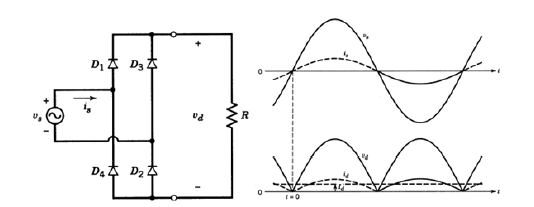
\includegraphics[scale=1]{imagenes/CA_CD.PNG} 
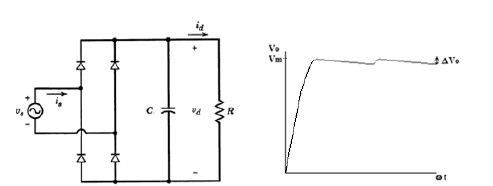
\includegraphics[scale=1]{imagenes/CA_CD1.PNG} 
\end{center}
\newpage
\begin{flushleft}
\section {Convertidor de potencia CD-CA}
\end{flushleft}
Los convertidores de corriente directa a corriente alterna son utilizados como controladores de motores así como fuentes de corriente alterna con modulación de frecuencia dependiendo el circuito. \\
Existen diversos tipos de convertidores inversores de los cuales el convertidor de una sola pierna y el convertidor en puente de media y onda completa, mostrados en las siguientes figuras son más comunes.\\
\linebreak
\linebreak
\begin{center}
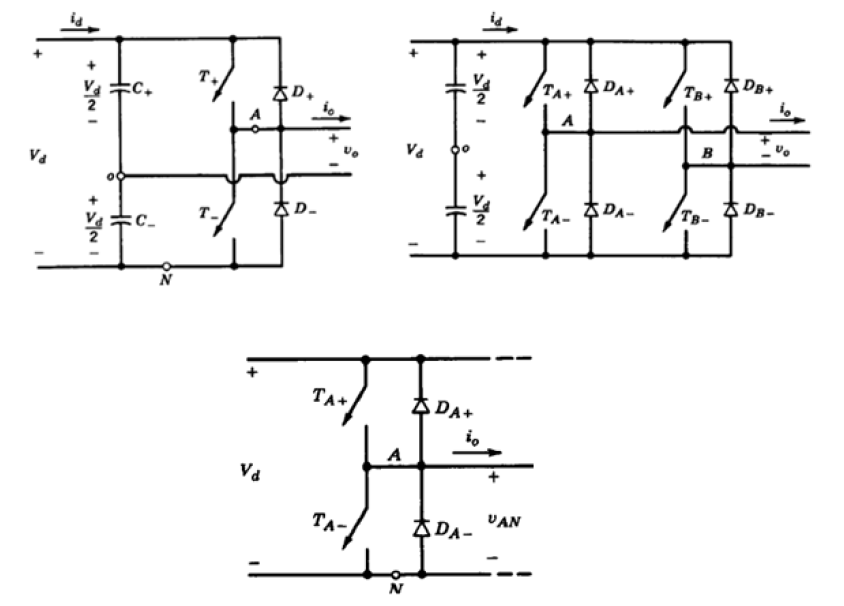
\includegraphics[scale=0.9]{imagenes/CD_CA.PNG} 
\end{center}
\newpage
\begin{flushleft}
\section{Convertidor de potencia CA-CA}
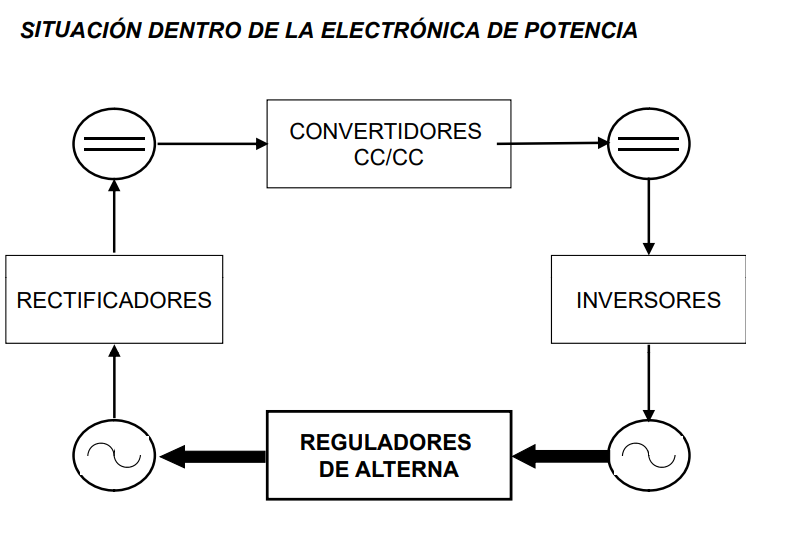
\includegraphics[scale=0.8]{imagenes/CA_CA.PNG} 
\end{flushleft}
\subsection{Características de los reguladores de alterna\\}
\begin{flushleft}
1. Realizan la conversión de AC-AC de forma directa y sin pasar por una intermedia de continua.\\
2. Los tiristores no necesitan bloqueo reforzado gracias al paso natural por cero de la intensidad.\\ 
3. Proporcionan una tensión de frecuencia fundamental menor o igual que la tensión de entrada.\\
4. Proporcionan una tensión con un cierto contenido de armónicos.\\ 
\subsection{Clasificación de los reguladores de alterna}
\end{flushleft}
\begin{flushleft}
* Totales\\
* Diferenciales\\
* De fase\\
* Integral \\
* Cicloconvertidores\\
\end{flushleft}
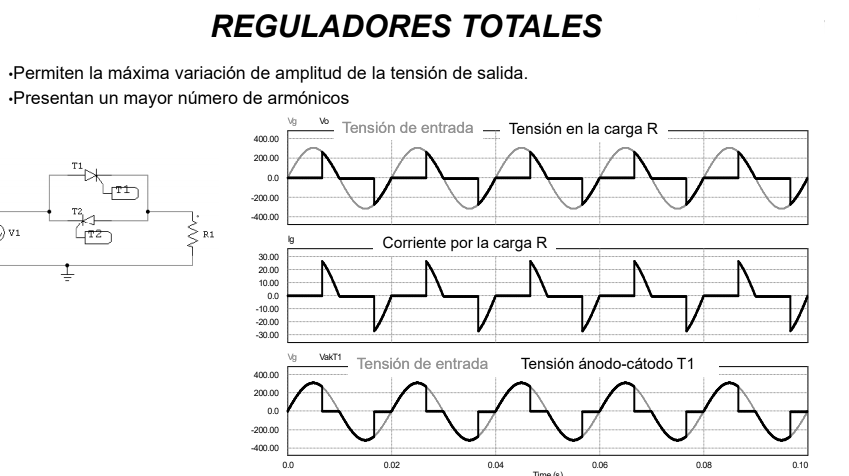
\includegraphics[scale=0.8]{imagenes/CA_CA_RT.PNG}\\
\linebreak
\linebreak
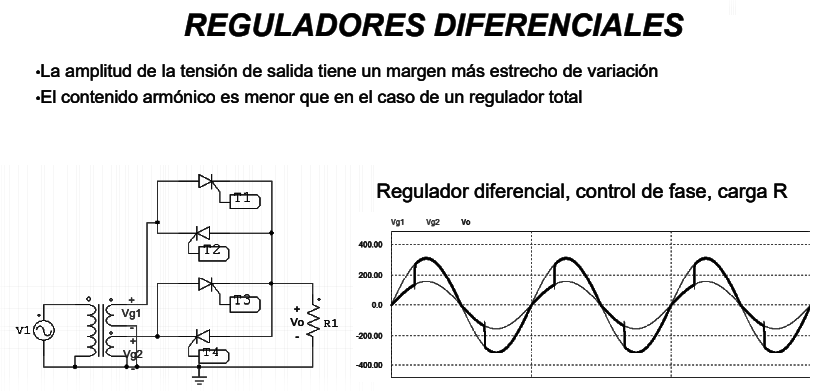
\includegraphics[scale=0.8]{imagenes/CA_CA_DIF.PNG}\\ 
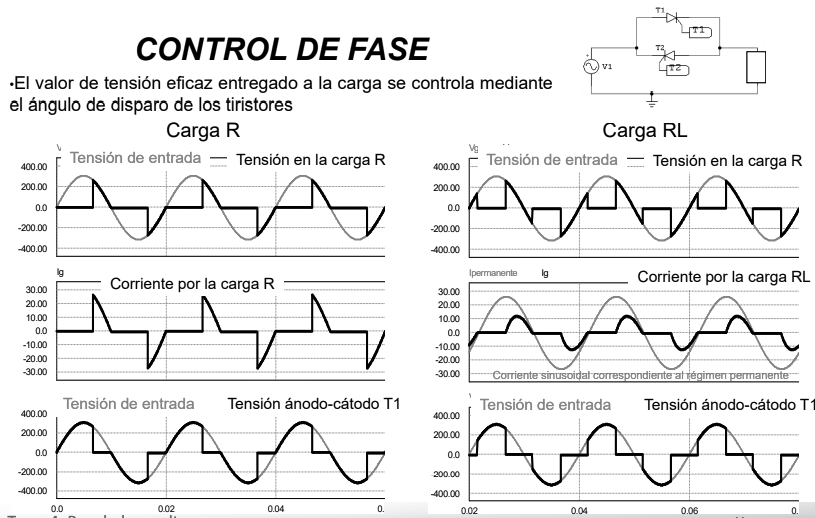
\includegraphics[scale=0.8]{imagenes/CA_CA_FAS.PNG} 
\linebreak
\linebreak
\linebreak
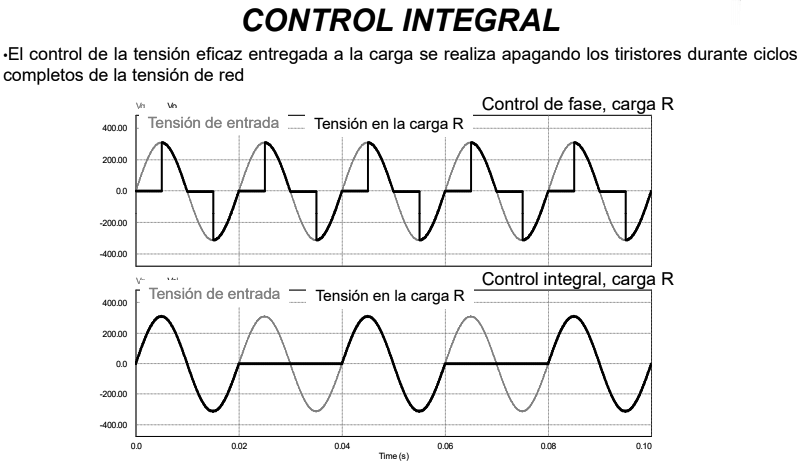
\includegraphics[scale=0.8]{imagenes/CA_CA_INT.PNG}
\newpage
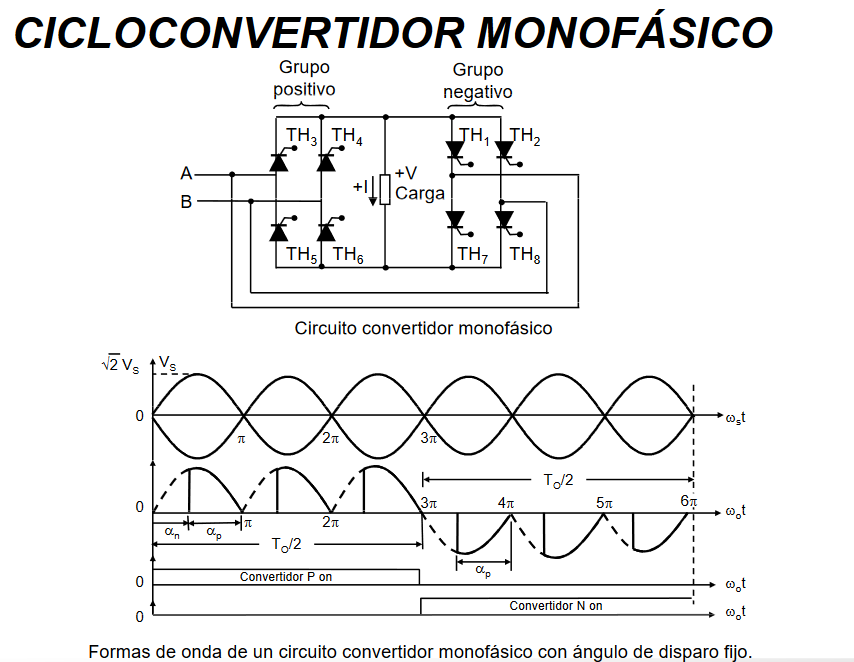
\includegraphics[scale=0.8]{imagenes/CA_CA_CI.PNG}
\linebreak
\linebreak
\begin{flushleft}
\section{Convertidores de potencia CD-CD}
\end{flushleft}
\begin{flushleft}
Los convertidores CD-CD se utilizan amplia mente en el control de los motores de tracción de los automóviles eléctricos, tranvias eléctricos, grúas marinas, montacargas y elevadores de minas.\\
Un convertidor se puede utilizar para elevar un voltaje de CD. Cuando el interruptor de Q se cierra durante el tiempo T1, la corriente del inductor se eleva y la energía se almacena en el inductor L. Si durante el T2 el interruptor se abre, la energía almacenada de el inductor se transfiere a la carga a través del diodo D y la corriente del inductor se abate.
\begin{center}
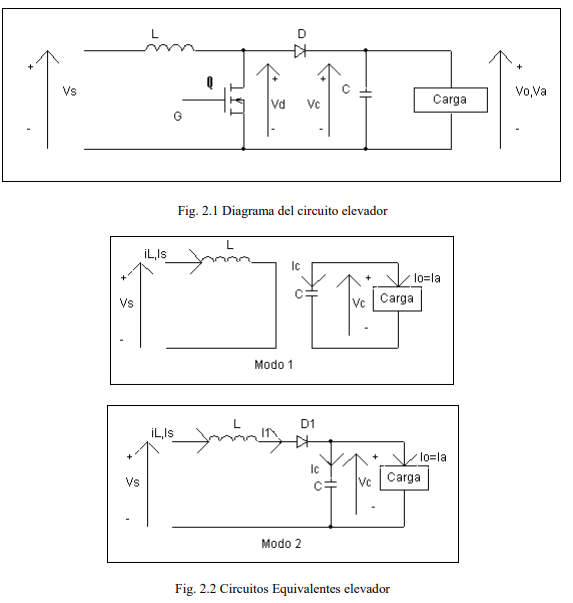
\includegraphics[scale=1.1]{imagenes/CD_CD.png} 
\end{center}
\newpage
La ecuación característica de este convertidor para determinar su voltaje de salida es: 
\begin{center}
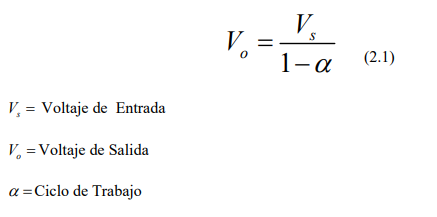
\includegraphics[scale=1]{imagenes/DC_DC1.PNG} 
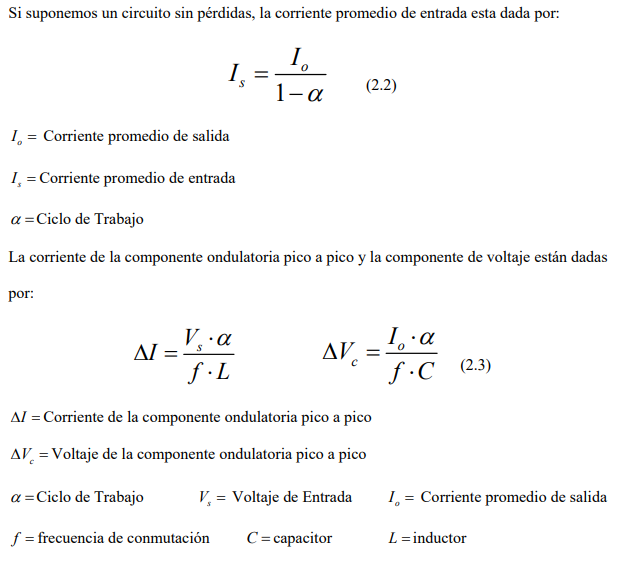
\includegraphics[scale=1]{imagenes/DC_DC2.PNG} 
\end{center}
\end{flushleft}
Son varios los tipos de convertidores DC-DC existentes.\\ Normalmente se clasifican en tres grupos: los que disminuyen la tensión a su salida (convertidor reductor), los que aumentan la tensión a su salida (convertidor elevador) y los que son capaces de realizar ambas funciones.\\
\newpage
\section{Conclusión}
\begin{flushleft}
Los convertidores entre tipos de corriente son muy importantes ya que están aplicados en prácticamente todos los dispositivos electrónicos y eléctricos que existen actualmente en todo tipo de campos imaginables por lo tanto el conocimiento del funcionamiento de cada uno de ellos es indispensable en cuanto a las bases que necesitaremos para continuar a lo largo de nuestra carrera en el desarrollo de sistemas electrónicos con diferentes fases de potencia.
\linebreak
\linebreak
\linebreak
\linebreak
\linebreak
\end{flushleft}
\section{Referencias Bibliográficas}
\begin{flushleft}
Carlos III. (2014). Conversion CA/CA. 17/09/19, de Universidad Carlos III,"http://ocw.uc3m.es/tecnologia-electronica/electronica-de-potencia/material-de-clase-1/MC-F-004.pdf" 
\linebreak
\linebreak
Martinez, V. (2015). CONVERTIDORES CD-CD . 17/09/19, de UDLA Sitio web: ocw.uc3m.es/tecnologia-electronica/electronica-de-potencia/material-de-clase-1/MC-F-004.pdf
\linebreak
\linebreak
Sector electricidad. (2015). ¿Qué son los armónicos y como nos afectan?. 17/09/19, de Sector electricidad Sitio web: "http://www.sectorelectricidad.com/13810/armonicos-que-son-y-como-nos-afectan/"
\linebreak 
\linebreak
\end{flushleft}
%\bibliographystyle{apalike} 
%\bibliography{biblio} 
%\cite{biblio}
\end{document}

\section{se}
